\documentclass[tikz]{standalone}
\usepackage{tikz}
\usetikzlibrary{patterns,arrows,calc,decorations.pathmorphing}
\usepackage{amsmath}
\usepackage{amsfonts}
\usepackage{amssymb}
\usepackage{enumitem}
\usetikzlibrary{shapes.geometric}
% Modified \textcircled macro
\renewcommand*\textcircled[1]{\tikz[baseline=(char.base)]{
  \node [shape=circle,draw,inner sep=1pt] (char) {#1};}}
%\renewcommand*\boxcenter{1.5}

%\newcommand{\brussel}[3]% [position, rotation], content
%{   \begin{tikzpicture}[overlay]
%	\draw [rotate=#3] (#1, #2) rectangle (#1+0.01, #2+0.02);  
% \draw [rotate= #3, blue, very thin] (#1-0.02,#2+0.02) arc (60:120:0.1);	
%\end{tikzpicture}
%}
\tikzset{
    partial ellipse/.style args={#1:#2:#3}{
        insert path={+ (#1:#3) arc (#1:#2:#3)}
    }
}

\begin{document}
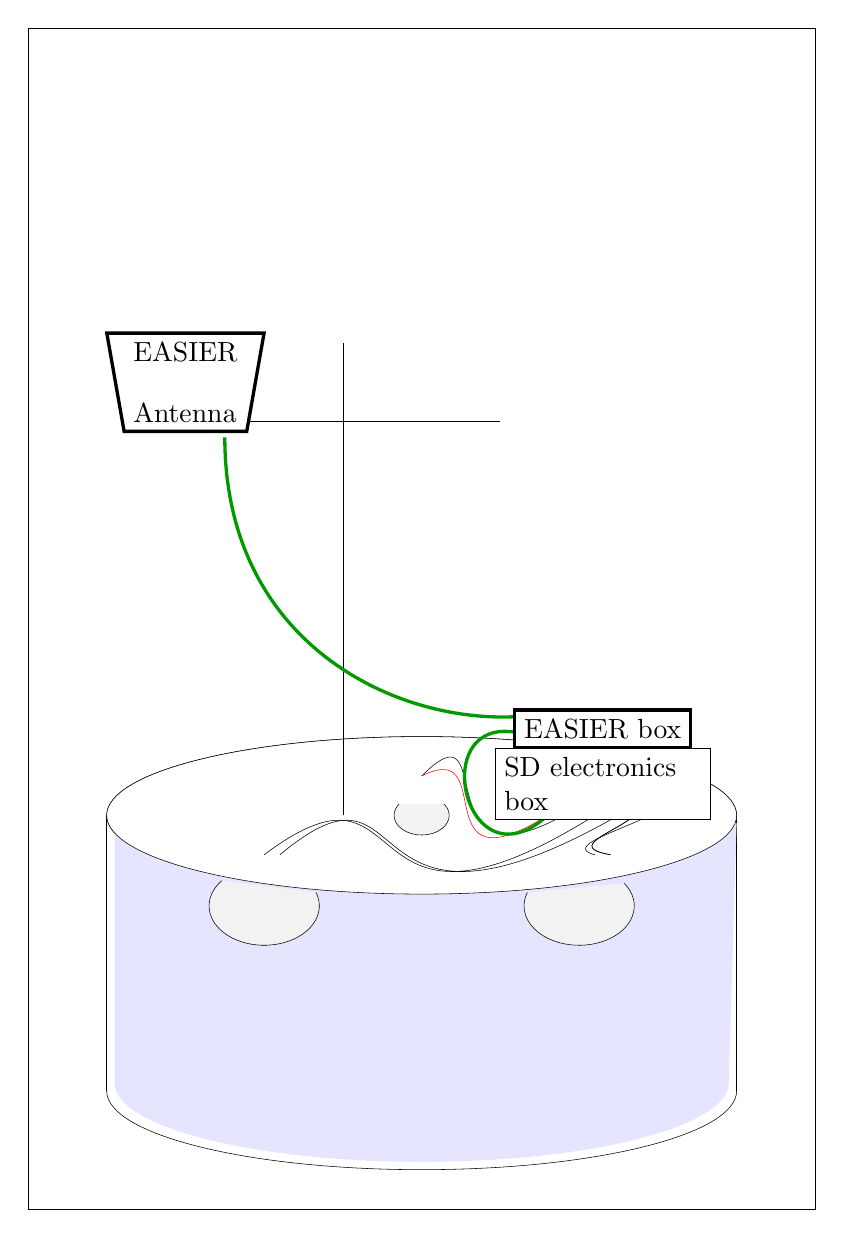
\begin{tikzpicture}
   	\draw [very thin] (0, 0) rectangle (10, 15);
%\draw  [very thin] (0.5,0.15) ellipse (0.4cm and 0.1cm);
\draw  [very thin] (5,5) ellipse (4cm and 1cm);
\draw  [very thin] (1,1.5) -- (1,5) ;
\draw  [very thin] (9,1.5) -- (9,5) ;
%\draw[thick, red, -latex] (0,0) [partial ellipse=30:150:3cm and 2cm];\
\draw  [very thin] (5,1.5) [partial ellipse=180:360:4cm and 1cm] ;
\fill[fill=blue!10]  (5,1.5+0.1) [partial ellipse=180:360:3.9cm and 1cm] -- (9, 5-0.1) -- (1+0.1,5-0.1)   ;
\filldraw  [fill=white, draw=black, very thin] (5,5) ellipse (4cm and 1cm);
\filldraw  [fill=gray!10, draw=black, very thin] (3,3.85) [partial ellipse=20:-220:0.7cm and 0.5cm] ;
\filldraw  [fill=gray!10, draw=black, very thin] (7,3.85) [partial ellipse=35:-200:0.7cm and 0.5cm] ;
\filldraw  [fill=gray!10, draw=black, very thin] (5,5) [partial ellipse=35:-215:0.35cm and 0.25cm] ;
\draw [very thin](6,5) -- (8,5) -- (8,5.5) -- (6,5.5) -- cycle;
\draw [very thin](4,5) -- (4,11);
\draw [very thin](1.5,10) -- (6,10);

\draw [very thin] (3,4.5) .. controls (5,6) and (4,3) .. (7.2,5);
\draw [very thin] (3.2,4.5) .. controls (5,6) and (4,3) .. (7.5,5);
\draw [very thin] (7.2,4.5) .. controls (6.8,4.6) and (7.5,4.8) .. (7.9,5);
\draw [very thin] (7.4,4.5) .. controls (6.8,4.6) and (7.5,4.8) .. (7.7,5);
\draw [very thin] (7.4,4.5) .. controls (6.8,4.6) and (7.5,4.8) .. (7.7,5);

\draw [very thin] (5,5.5) .. controls (6,6.5) and (5,4) .. (6.8,5);
\draw [very thin, red] (5,5.5) .. controls (6,6) and (5,4) .. (6.6,5);

%\draw [black] (3,9.5) -- (2.5,11) -- (3.8,12) -- ();

\node  [very thick,fill=white,trapezium, trapezium angle=-80,draw, align=left] at (2,10.5) {EASIER \\[1em] Antenna};
\draw [very thick, black!40!green] (2.5,9.8) .. controls (2.5,7) and (5,6) .. (6.6,6.3);
\draw [very thick, black!40!green] (6.4,6.0) .. controls (5,6.5) and (5.5,4) .. (6.6,5);


\node[draw,fill=white,text width=2.5cm,minimum height=2mm] at (7.3,5.4) {SD electronics box};
\node[draw,very thick, fill=white,text width=2cm,minimum height=2mm] at (7.3,6.1) {EASIER box};


   \end{tikzpicture}
\end{document}